\newpage

\section{HIGH10}
%\begin{table}
	\centering
%	\begingroup
	\fontsize{9}{9}
	\selectfont
	\begin{tabular}{lr}
		\toprule
		Ticker            & Volatility \\
		\midrule
		\textbf{GOLL4.SA} & 0.0741696  \\
		\textbf{USIM5.SA} & 0.0592991  \\
		\textbf{RAIL3.SA} & 0.0541754  \\
		\textbf{CSNA3.SA} & 0.0523774  \\
		\textbf{GOAU4.SA} & 0.0505415  \\
		\textbf{MULT3.SA} & 0.0171126  \\
		\textbf{RADL3.SA} & 0.0168716  \\
		\textbf{EQTL3.SA} & 0.0150024  \\
		\textbf{EGIE3.SA} & 0.0137375  \\
		\textbf{ABEV3.SA} & 0.0136296  \\
		\bottomrule
	\end{tabular} \caption{Annualized Returns: Jan20 - Jun22}
	\label{tab:StocksVol}  % LEMBRE-SE DE MUDAR O LABEL
%	\endgroup{}
\end{table}

\begin{figure}[H]
	%\begin{adjustwidth}{2.2cm}{2.2cm}
	\begin{subfigmatrix}{2}
		\subfigure[Weigths]{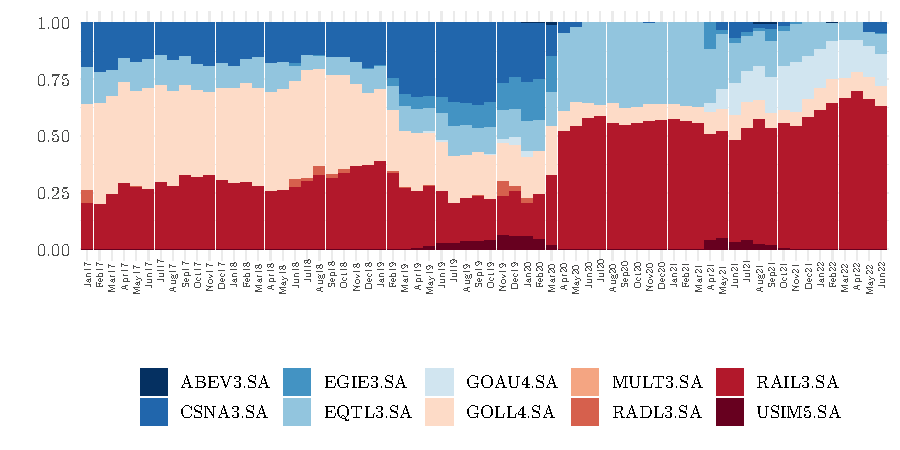
\includegraphics{figures/totalWeigthMVPVol.pdf}}
		\subfigure[Risks]{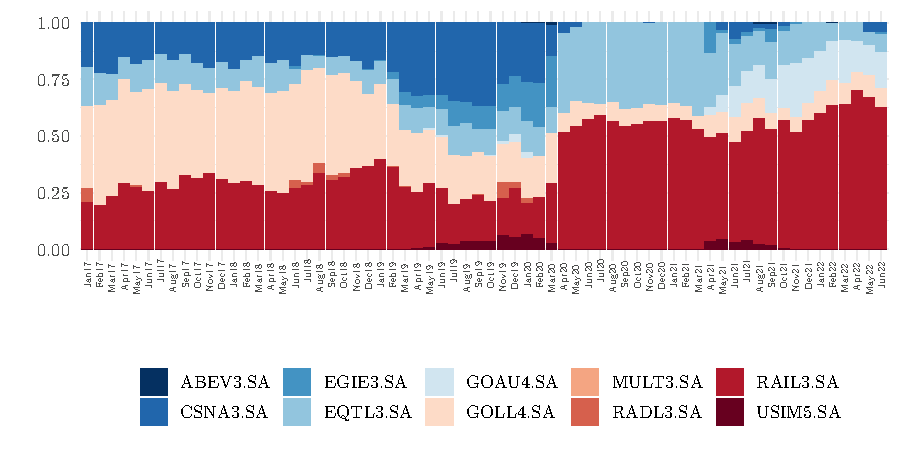
\includegraphics{figures/totalRiskMVPVol.pdf}}
	\end{subfigmatrix}
	\caption{Monthly distribution of MVP.}
	\label{fig:totalRiskMVP}
	%\end{adjustwidth}
\end{figure}


% A RPP has the weights distributed with the purpose of having a uniform risk distribution, Figure \ref{fig:totalRiskPPP} shows the distribution of weights and risks in our backtest study.

\begin{figure}[H]
	%\begin{adjustwidth}{2.2cm}{2.2cm}
	\begin{subfigmatrix}{2}
		\subfigure[Weigths]{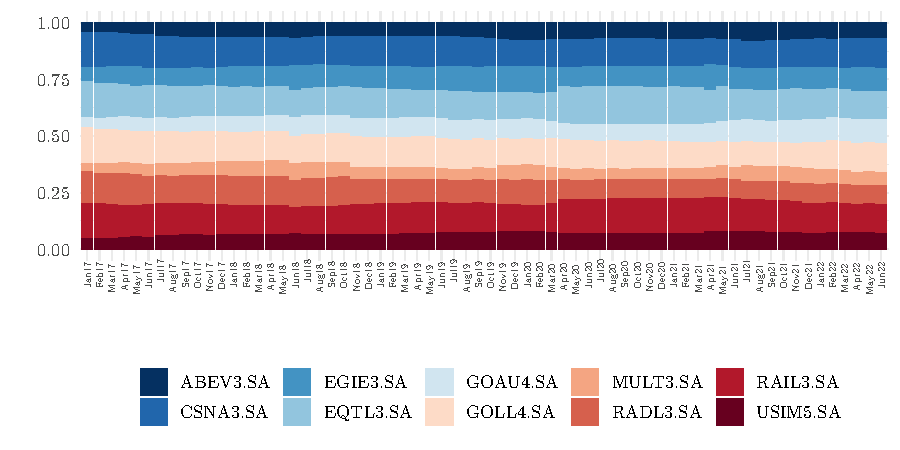
\includegraphics{figures/totalWeigthRPPVol.pdf}}
		\subfigure[Risks]{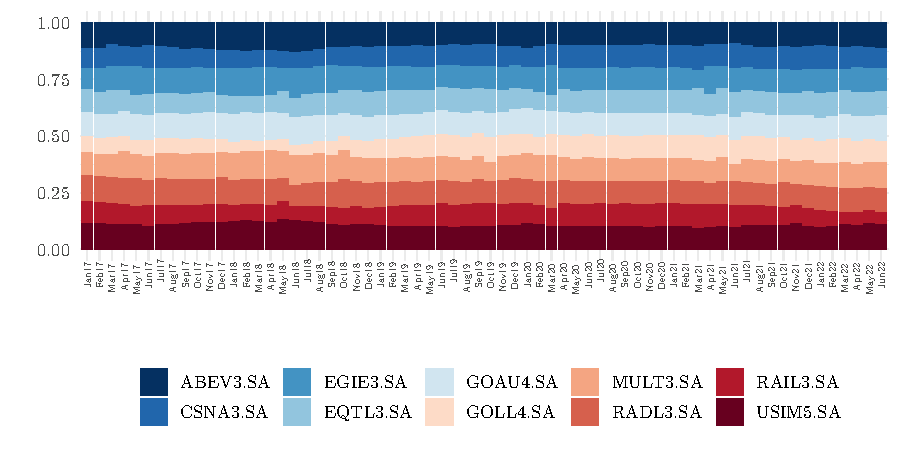
\includegraphics{figures/totalRiskRPPVol.pdf}}
	\end{subfigmatrix}
	\caption{Monthly distribution of RPP.}
	\label{fig:totalRiskPPP}
	%\end{adjustwidth}
\end{figure}

% The total return of the RPP was greater than the MVP in the period studied. While MVP had a total return of 52\%, the accumulated RPP return was 119\% (44\% higher than the MVP).

\begin{figure}[H]
	\centering
	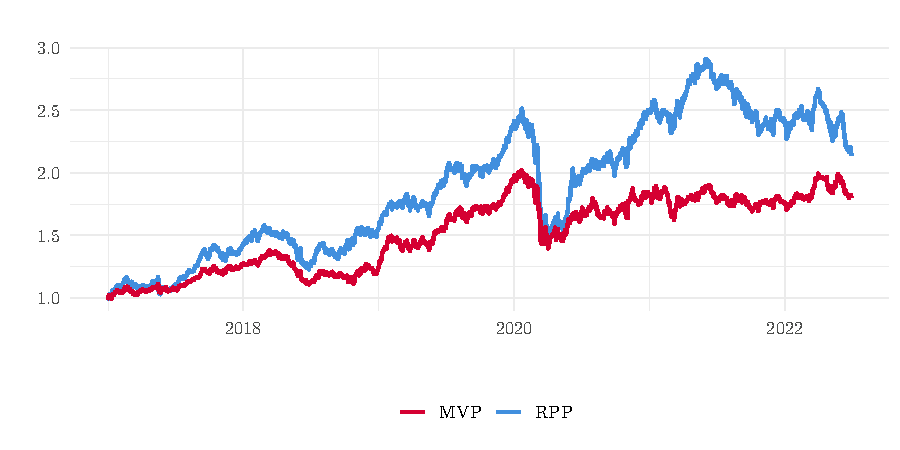
\includegraphics{figures/retornoRPPMVPVol.pdf}
	\caption{MVP and RPP accumulated returns: January 2017 $-$ June 2022.}
	\label{fig:retornoRPPMVP}
\end{figure}

% The MVP volatility was slightly smaller than the RPP. However, considering the zero risk-free rate, the RRP Sharpe ratio was bigger than the MVP.

\begin{table}
    \centering
      \begingroup
      \fontsize{9}{9}
      \selectfont 
\begin{tabular}{>{}lrr}
\toprule
  & MVP & RPP\\
\midrule
\textbf{Annualized Return} & 0.1149 & 0.1502\\
\textbf{Annualized Std Dev} & 0.2113 & 0.2570\\
\textbf{Annualized Sharpe (Rf=0\%)} & 0.5437 & 0.5846\\
\bottomrule
\end{tabular} \caption{Annualized Returns: Jan17 - Jun22}
      \label{tab:RPPVol}  % LEMBRE-SE DE MUDAR O LABEL
      \endgroup{}
      \end{table}


% We remind that after 2020, due to the COVID-19 pandemic, the volatility of all assets has exploded, so we separate two period in our study, from 2017 until 2019 and after 2020. We may observe that the RPP performed much better (135\% gain) than the MVP (79\% gain) in the period between January 2017 and December 2019. Besides, MVP had a great annualized Sharpe ratio of 1.20, however, lower than RPP annualized Sharpe ratio (1.58).

\begin{table}
    \centering
      \begingroup
      \fontsize{9}{9}
      \selectfont 
\begin{tabular}{>{}lrr}
\toprule
  & MVP & RPP\\
\midrule
\textbf{Annualized Return} & 0.2472 & 0.3343\\
\textbf{Annualized Std Dev} & 0.1585 & 0.1983\\
\textbf{Annualized Sharpe (Rf=0\%)} & 1.5594 & 1.6860\\
\bottomrule
\end{tabular} \caption{Annualized Returns: Jan20 - Dez19}
      \label{tab:RPPVol1}  % LEMBRE-SE DE MUDAR O LABEL
      \endgroup{}
      \end{table}

\begin{figure}[H]
	%\begin{adjustwidth}{2.2cm}{2.2cm}
	\begin{subfigmatrix}{2}
		\subfigure[January 2017 $-$ December 2019.]{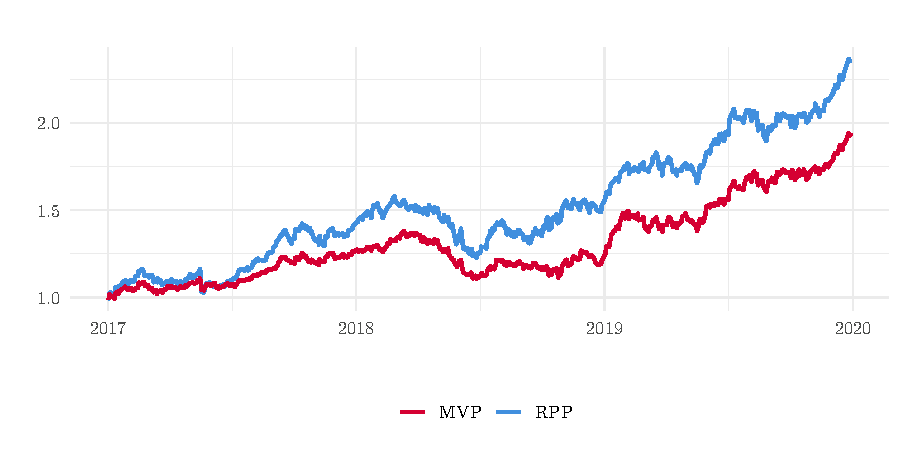
\includegraphics{figures/retornoRPPMVPVol1.pdf}}
		\subfigure[January 2020 $-$ June 2022.]{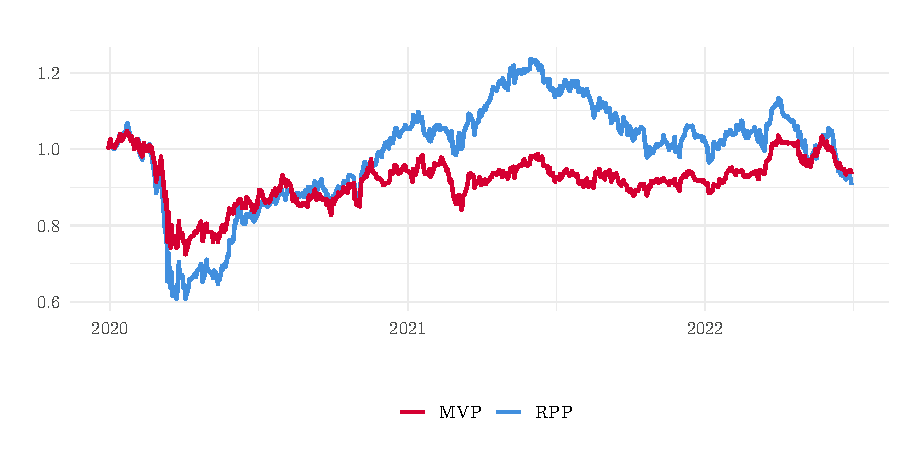
\includegraphics{figures/retornoRPPMVPVol2.pdf}}
	\end{subfigmatrix}
	\caption{MVP and RPP accumulated returns.}
	\label{fig:retornoRPPMVP12}
	%\end{adjustwidth}
\end{figure}

% From January 2020 to June 2022, MVP exhibited an accumulated $15.2\%$ loss, while RPP reduced the loss to only $6.8\%$. Despite the loss in the period, the RPP improved the protection of the invested capital.

\begin{table}
    \centering
      \begingroup
      \fontsize{9}{9}
      \selectfont 
\begin{tabular}{>{}lrr}
\toprule
  & MVP & RPP\\
\midrule
\textbf{Annualized Return} & -0.0265 & -0.0386\\
\textbf{Annualized Std Dev} & 0.2611 & 0.3135\\
\textbf{Annualized Sharpe (Rf=0\%)} & -0.1016 & -0.1232\\
\bottomrule
\end{tabular} \caption{Annualized Returns: Jan20 - Jun22}
      \label{tab:RPPVol2}  % LEMBRE-SE DE MUDAR O LABEL
      \endgroup{}
      \end{table}

% In our study, the RPP had a superior performance when compared to the MVP, both in high and low moments. Clearly, this study is not conclusive, but simply an example of the use of Algorithm~\ref{Alg:GeneralSeach}.


\newpage

\section{volHighLow Volatility}
%\begin{table}
	\centering
%	\begingroup
	\fontsize{9}{9}
	\selectfont
	\begin{tabular}{lr}
		\toprule
		Ticker            & Volatility \\
		\midrule
		\textbf{GOLL4.SA} & 0.0741696  \\
		\textbf{USIM5.SA} & 0.0592991  \\
		\textbf{RAIL3.SA} & 0.0541754  \\
		\textbf{CSNA3.SA} & 0.0523774  \\
		\textbf{GOAU4.SA} & 0.0505415  \\
		\textbf{MULT3.SA} & 0.0171126  \\
		\textbf{RADL3.SA} & 0.0168716  \\
		\textbf{EQTL3.SA} & 0.0150024  \\
		\textbf{EGIE3.SA} & 0.0137375  \\
		\textbf{ABEV3.SA} & 0.0136296  \\
		\bottomrule
	\end{tabular} \caption{Annualized Returns: Jan20 - Jun22}
	\label{tab:StocksVol}  % LEMBRE-SE DE MUDAR O LABEL
%	\endgroup{}
\end{table}

\begin{figure}[H]
	%\begin{adjustwidth}{2.2cm}{2.2cm}
	\begin{subfigmatrix}{2}
		\subfigure[Weigths]{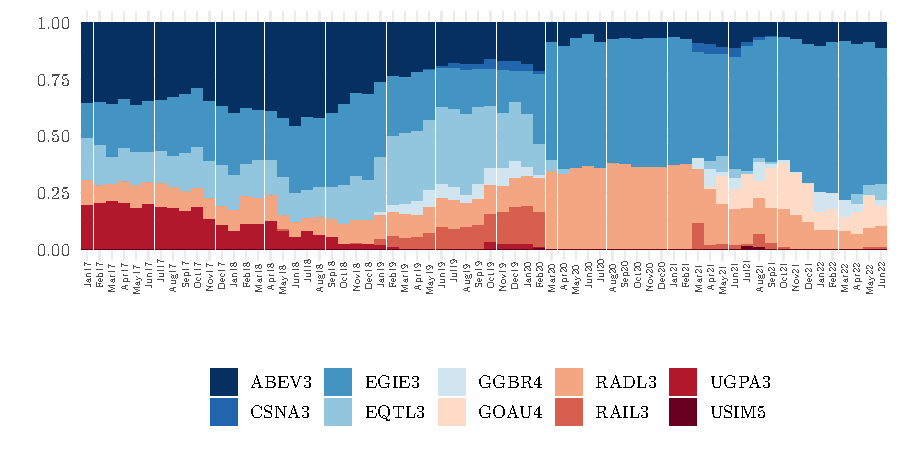
\includegraphics{figures/WeigthMVPvolHighLow.pdf}}
		\subfigure[Risks]{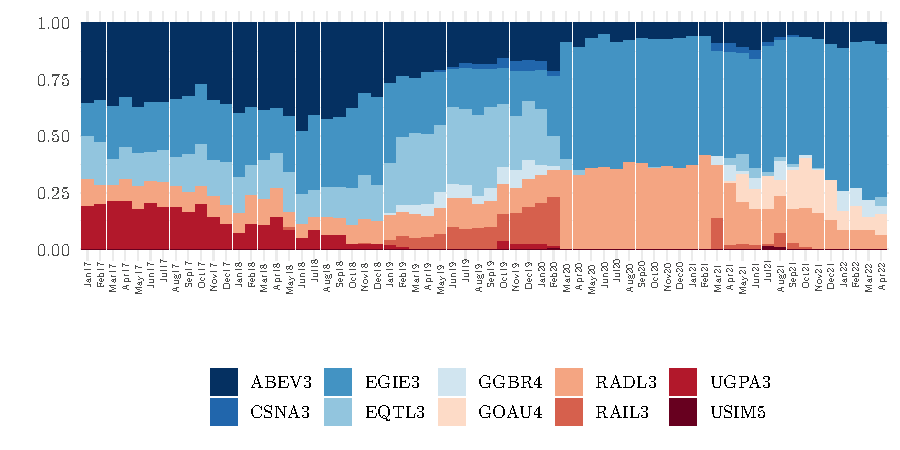
\includegraphics{figures/RiskMVPvolHighLow.pdf}}
	\end{subfigmatrix}
	\caption{Monthly distribution of MVP.}
	\label{fig:totalRiskMVP}
	%\end{adjustwidth}
\end{figure}


% A RPP has the weights distributed with the purpose of having a uniform risk distribution, Figure \ref{fig:totalRiskPPP} shows the distribution of weights and risks in our backtest study.

\begin{figure}[H]
	%\begin{adjustwidth}{2.2cm}{2.2cm}
	\begin{subfigmatrix}{2}
		\subfigure[Weigths]{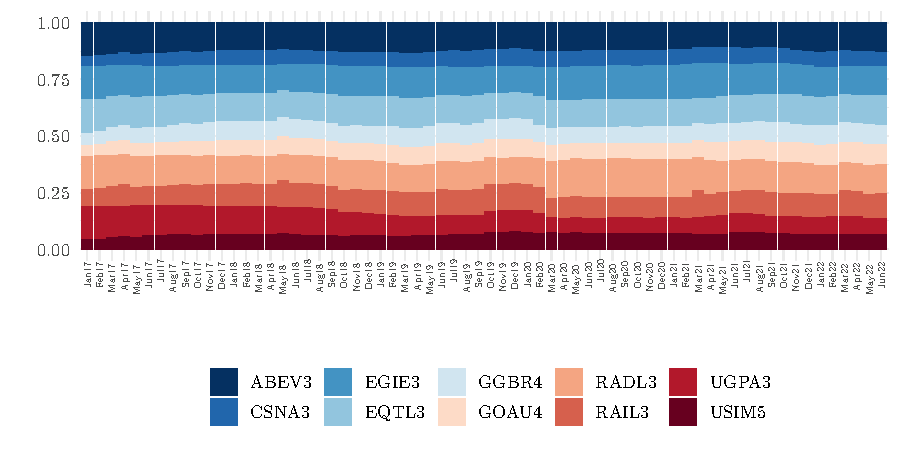
\includegraphics{figures/WeigthRPPvolHighLow.pdf}}
		\subfigure[Risks]{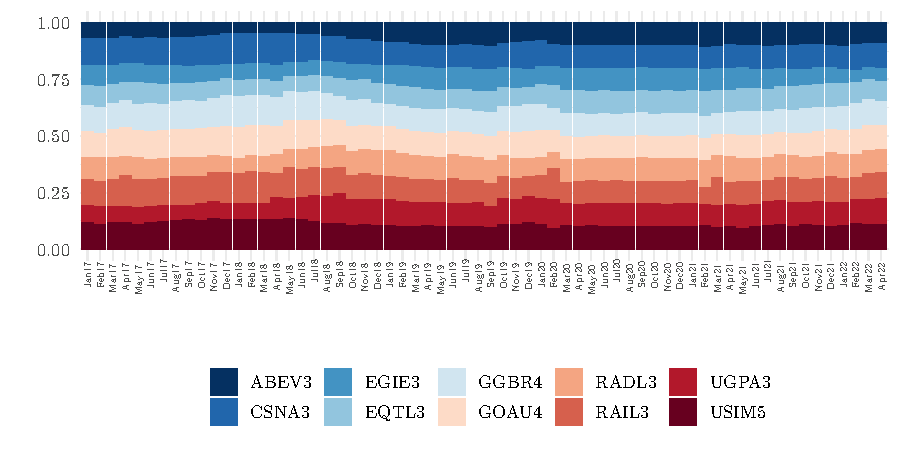
\includegraphics{figures/RiskRPPvolHighLow.pdf}}
	\end{subfigmatrix}
	\caption{Monthly distribution of RPP.}
	\label{fig:totalRiskPPP}
	%\end{adjustwidth}
\end{figure}

% The total return of the RPP was greater than the MVP in the period studied. While MVP had a total return of 52\%, the accumulated RPP return was 119\% (44\% higher than the MVP).

\begin{figure}[H]
	\centering
	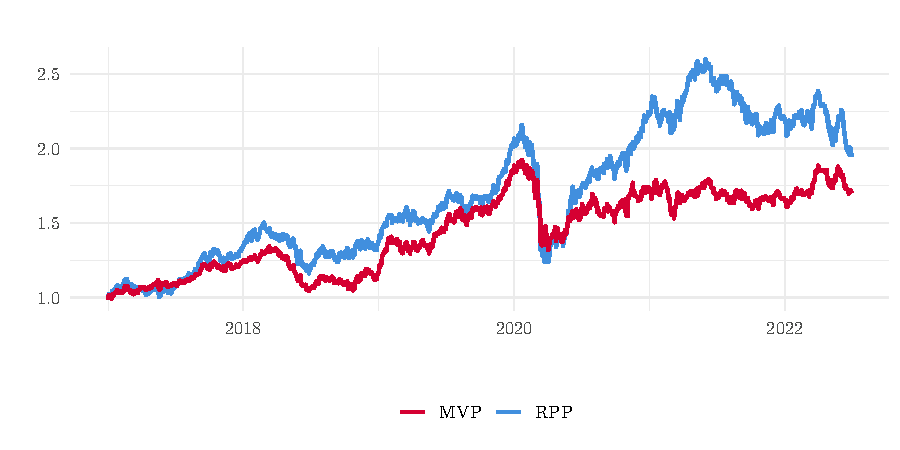
\includegraphics{figures/retornovolHighLow.pdf}
	\caption{MVP and RPP accumulated returns: January 2017 $-$ June 2022.}
	\label{fig:retornoRPPMVP}
\end{figure}

% The MVP volatility was slightly smaller than the RPP. However, considering the zero risk-free rate, the RRP Sharpe ratio was bigger than the MVP.

\begin{table}
	\centering
	\begingroup
	\fontsize{9}{9}
	\selectfont
	\begin{tabular}{>{}lrr}
		\toprule
		                                    & MVP    & RPP    \\
		\midrule
		\textbf{Annualized Return}          & 0.1029 & 0.1310 \\
		\textbf{Annualized Std Dev}         & 0.2115 & 0.2544 \\
		\textbf{Annualized Sharpe (Rf=0\%)} & 0.4864 & 0.5147 \\
		\bottomrule
	\end{tabular} \caption{Annualized Returns: Jan17 - Jun22}
	\label{tab: HighLow }
	\endgroup{}
\end{table}


% We remind that after 2020, due to the COVID-19 pandemic, the volatility of all assets has exploded, so we separate two period in our study, from 2017 until 2019 and after 2020. We may observe that the RPP performed much better (135\% gain) than the MVP (79\% gain) in the period between January 2017 and December 2019. Besides, MVP had a great annualized Sharpe ratio of 1.20, however, lower than RPP annualized Sharpe ratio (1.58).

\begin{table}
      \centering
      \begingroup
      \fontsize{9}{9}
      \selectfont 
\begin{tabular}{>{}lrr}
\toprule
  & MVP & RPP\\
\midrule
\textbf{Annualized Return} & 0.2271 & 0.2658\\
\textbf{Annualized Std Dev} & 0.1582 & 0.1933\\
\textbf{Annualized Sharpe (Rf=0\%)} & 1.4353 & 1.3754\\
\bottomrule
\end{tabular} \caption{Annualized Returns: Jan17 - Dez19}
      \label{tab: HighLow1 }  
      \endgroup{}
      \end{table}

\begin{figure}[H]
	%\begin{adjustwidth}{2.2cm}{2.2cm}
	\begin{subfigmatrix}{2}
		\subfigure[January 2017 $-$ December 2019.]{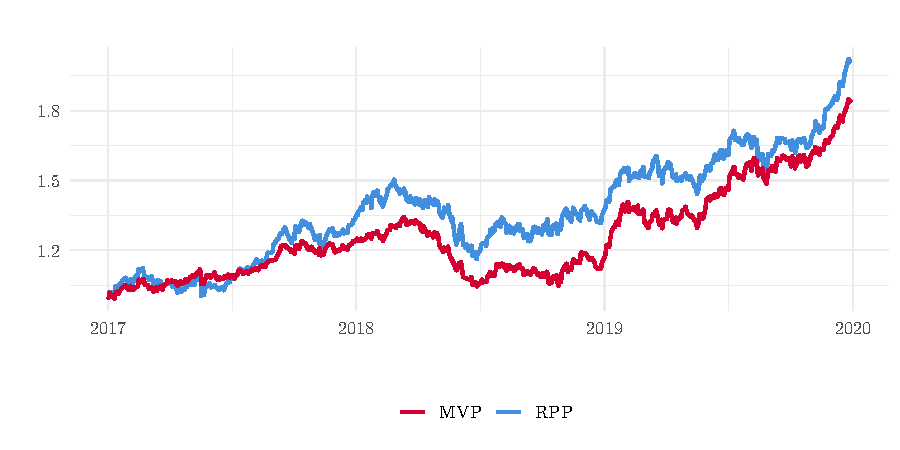
\includegraphics{figures/retornovolHighLow1.pdf}}
		\subfigure[January 2020 $-$ June 2022.]{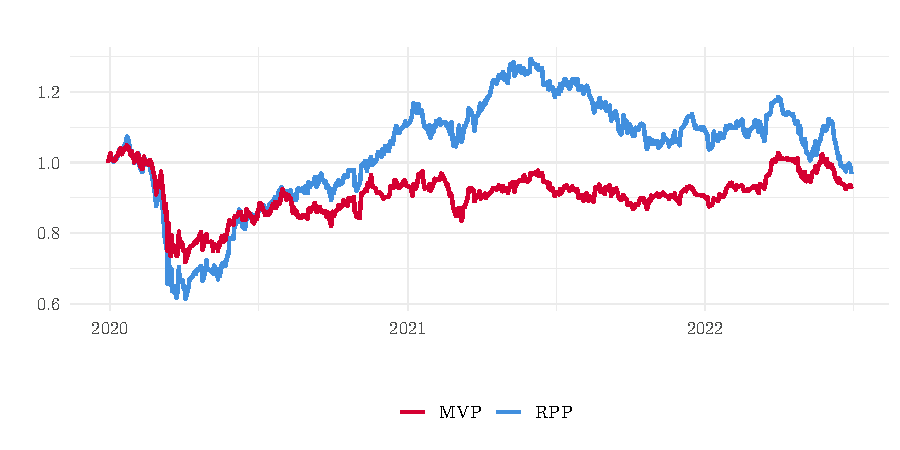
\includegraphics{figures/retornovolHighLow2.pdf}}
	\end{subfigmatrix}
	\caption{MVP and RPP accumulated returns.}
	\label{fig:retornoRPPMVP12}
	%\end{adjustwidth}
\end{figure}

% From January 2020 to June 2022, MVP exhibited an accumulated $15.2\%$ loss, while RPP reduced the loss to only $6.8\%$. Despite the loss in the period, the RPP improved the protection of the invested capital.

\begin{table}[H]
      \centering
      \begingroup
      \fontsize{9}{9}
      \selectfont 
\begin{tabular}{>{}lrr}
\toprule
  & MVP & RPP\\
\midrule
\textbf{Annualized Return} & -0.0305 & -0.0130\\
\textbf{Annualized Std Dev} & 0.2619 & 0.3128\\
\textbf{Annualized Sharpe (Rf=0\%)} & -0.1165 & -0.0415\\
\bottomrule
\end{tabular} \caption{Annualized Returns: Jan20 - Jun22}
      \label{tab: HighLow2 }  
      \endgroup{}
      \end{table}

% In our study, the RPP had a superior performance when compared to the MVP, both in high and low moments. Clearly, this study is not conclusive, but simply an example of the use of Algorithm~\ref{Alg:GeneralSeach}.

\newpage

\section{volHighLow Volatility}
%\begin{table}
	\centering
%	\begingroup
	\fontsize{9}{9}
	\selectfont
	\begin{tabular}{lr}
		\toprule
		Ticker            & Volatility \\
		\midrule
		\textbf{GOLL4.SA} & 0.0741696  \\
		\textbf{USIM5.SA} & 0.0592991  \\
		\textbf{RAIL3.SA} & 0.0541754  \\
		\textbf{CSNA3.SA} & 0.0523774  \\
		\textbf{GOAU4.SA} & 0.0505415  \\
		\textbf{MULT3.SA} & 0.0171126  \\
		\textbf{RADL3.SA} & 0.0168716  \\
		\textbf{EQTL3.SA} & 0.0150024  \\
		\textbf{EGIE3.SA} & 0.0137375  \\
		\textbf{ABEV3.SA} & 0.0136296  \\
		\bottomrule
	\end{tabular} \caption{Annualized Returns: Jan20 - Jun22}
	\label{tab:StocksVol}  % LEMBRE-SE DE MUDAR O LABEL
%	\endgroup{}
\end{table}

\begin{figure}[H]
	%\begin{adjustwidth}{2.2cm}{2.2cm}
	\begin{subfigmatrix}{2}
		\subfigure[Weigths]{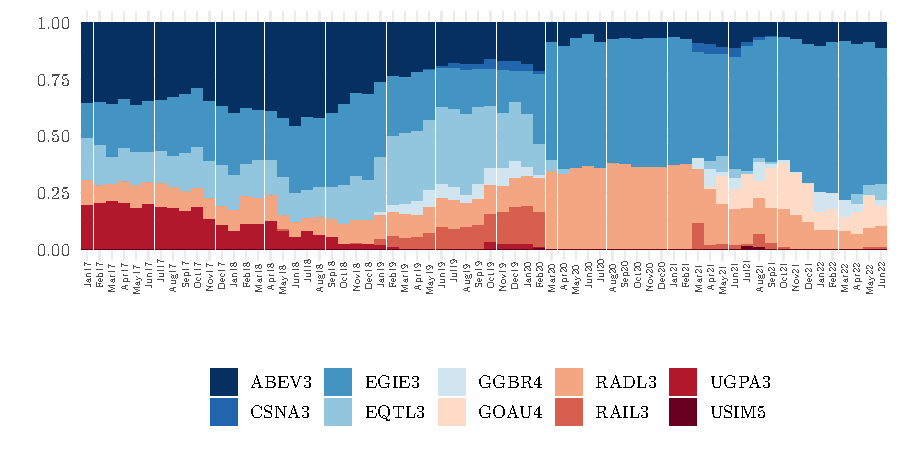
\includegraphics{figures/WeigthMVPvolHighLow.pdf}}
		\subfigure[Risks]{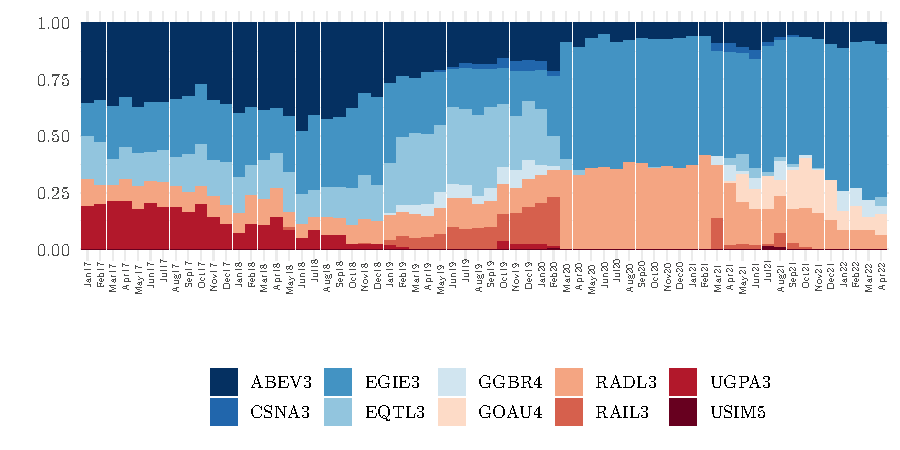
\includegraphics{figures/RiskMVPvolHighLow.pdf}}
	\end{subfigmatrix}
	\caption{Monthly distribution of MVP.}
	\label{fig:totalRiskMVP}
	%\end{adjustwidth}
\end{figure}


% A RPP has the weights distributed with the purpose of having a uniform risk distribution, Figure \ref{fig:totalRiskPPP} shows the distribution of weights and risks in our backtest study.

\begin{figure}[H]
	%\begin{adjustwidth}{2.2cm}{2.2cm}
	\begin{subfigmatrix}{2}
		\subfigure[Weigths]{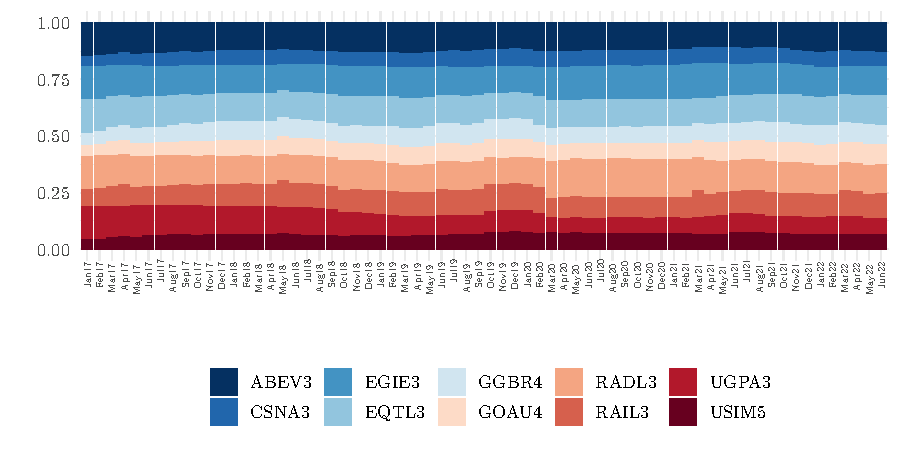
\includegraphics{figures/WeigthRPPvolHighLow.pdf}}
		\subfigure[Risks]{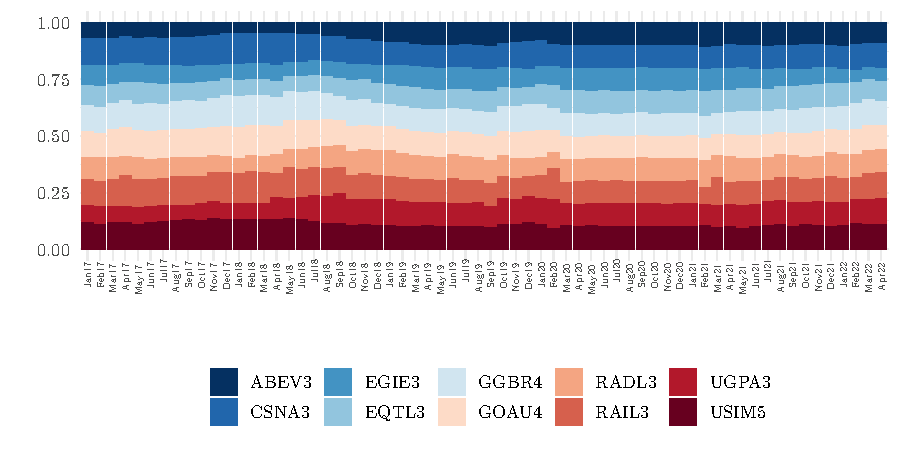
\includegraphics{figures/RiskRPPvolHighLow.pdf}}
	\end{subfigmatrix}
	\caption{Monthly distribution of RPP.}
	\label{fig:totalRiskPPP}
	%\end{adjustwidth}
\end{figure}

% The total return of the RPP was greater than the MVP in the period studied. While MVP had a total return of 52\%, the accumulated RPP return was 119\% (44\% higher than the MVP).

\begin{figure}[H]
	\centering
	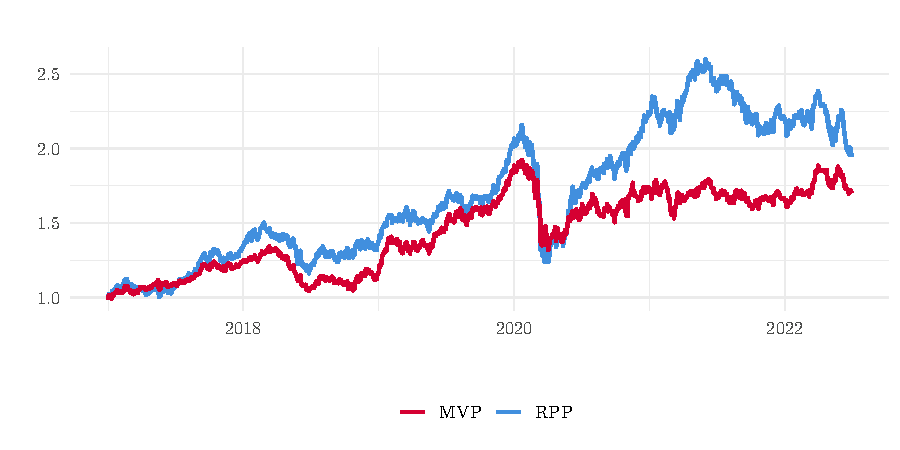
\includegraphics{figures/retornovolHighLow.pdf}
	\caption{MVP and RPP accumulated returns: January 2017 $-$ June 2022.}
	\label{fig:retornoRPPMVP}
\end{figure}

% The MVP volatility was slightly smaller than the RPP. However, considering the zero risk-free rate, the RRP Sharpe ratio was bigger than the MVP.

\begin{table}
	\centering
	\begingroup
	\fontsize{9}{9}
	\selectfont
	\begin{tabular}{>{}lrr}
		\toprule
		                                    & MVP    & RPP    \\
		\midrule
		\textbf{Annualized Return}          & 0.1029 & 0.1310 \\
		\textbf{Annualized Std Dev}         & 0.2115 & 0.2544 \\
		\textbf{Annualized Sharpe (Rf=0\%)} & 0.4864 & 0.5147 \\
		\bottomrule
	\end{tabular} \caption{Annualized Returns: Jan17 - Jun22}
	\label{tab: HighLow }
	\endgroup{}
\end{table}


% We remind that after 2020, due to the COVID-19 pandemic, the volatility of all assets has exploded, so we separate two period in our study, from 2017 until 2019 and after 2020. We may observe that the RPP performed much better (135\% gain) than the MVP (79\% gain) in the period between January 2017 and December 2019. Besides, MVP had a great annualized Sharpe ratio of 1.20, however, lower than RPP annualized Sharpe ratio (1.58).

\begin{table}
      \centering
      \begingroup
      \fontsize{9}{9}
      \selectfont 
\begin{tabular}{>{}lrr}
\toprule
  & MVP & RPP\\
\midrule
\textbf{Annualized Return} & 0.2271 & 0.2658\\
\textbf{Annualized Std Dev} & 0.1582 & 0.1933\\
\textbf{Annualized Sharpe (Rf=0\%)} & 1.4353 & 1.3754\\
\bottomrule
\end{tabular} \caption{Annualized Returns: Jan17 - Dez19}
      \label{tab: HighLow1 }  
      \endgroup{}
      \end{table}

\begin{figure}[H]
	%\begin{adjustwidth}{2.2cm}{2.2cm}
	\begin{subfigmatrix}{2}
		\subfigure[January 2017 $-$ December 2019.]{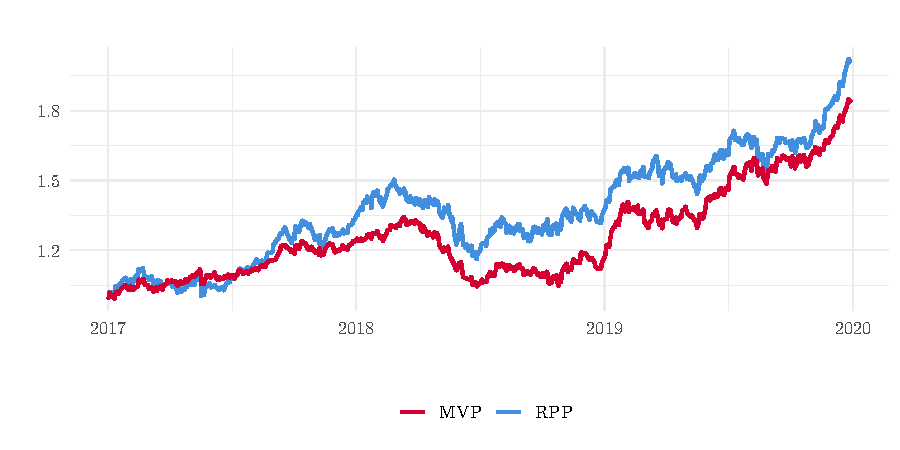
\includegraphics{figures/retornovolHighLow1.pdf}}
		\subfigure[January 2020 $-$ June 2022.]{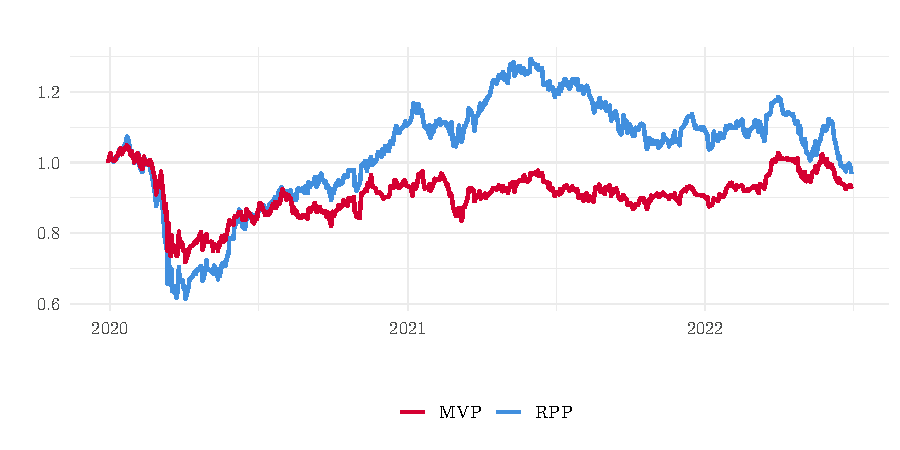
\includegraphics{figures/retornovolHighLow2.pdf}}
	\end{subfigmatrix}
	\caption{MVP and RPP accumulated returns.}
	\label{fig:retornoRPPMVP12}
	%\end{adjustwidth}
\end{figure}

% From January 2020 to June 2022, MVP exhibited an accumulated $15.2\%$ loss, while RPP reduced the loss to only $6.8\%$. Despite the loss in the period, the RPP improved the protection of the invested capital.

\begin{table}[H]
      \centering
      \begingroup
      \fontsize{9}{9}
      \selectfont 
\begin{tabular}{>{}lrr}
\toprule
  & MVP & RPP\\
\midrule
\textbf{Annualized Return} & -0.0305 & -0.0130\\
\textbf{Annualized Std Dev} & 0.2619 & 0.3128\\
\textbf{Annualized Sharpe (Rf=0\%)} & -0.1165 & -0.0415\\
\bottomrule
\end{tabular} \caption{Annualized Returns: Jan20 - Jun22}
      \label{tab: HighLow2 }  
      \endgroup{}
      \end{table}

% In our study, the RPP had a superior performance when compared to the MVP, both in high and low moments. Clearly, this study is not conclusive, but simply an example of the use of Algorithm~\ref{Alg:GeneralSeach}.

% \newpage

% \section{LOW}
% %\begin{table}
	\centering
%	\begingroup
	\fontsize{9}{9}
	\selectfont
	\begin{tabular}{lr}
		\toprule
		Ticker            & Volatility \\
		\midrule
		\textbf{GOLL4.SA} & 0.0741696  \\
		\textbf{USIM5.SA} & 0.0592991  \\
		\textbf{RAIL3.SA} & 0.0541754  \\
		\textbf{CSNA3.SA} & 0.0523774  \\
		\textbf{GOAU4.SA} & 0.0505415  \\
		\textbf{MULT3.SA} & 0.0171126  \\
		\textbf{RADL3.SA} & 0.0168716  \\
		\textbf{EQTL3.SA} & 0.0150024  \\
		\textbf{EGIE3.SA} & 0.0137375  \\
		\textbf{ABEV3.SA} & 0.0136296  \\
		\bottomrule
	\end{tabular} \caption{Annualized Returns: Jan20 - Jun22}
	\label{tab:StocksVol}  % LEMBRE-SE DE MUDAR O LABEL
%	\endgroup{}
\end{table}

% \begin{figure}[H]
% 	%\begin{adjustwidth}{2.2cm}{2.2cm}
% 	\begin{subfigmatrix}{2}
% 		\subfigure[Weigths]{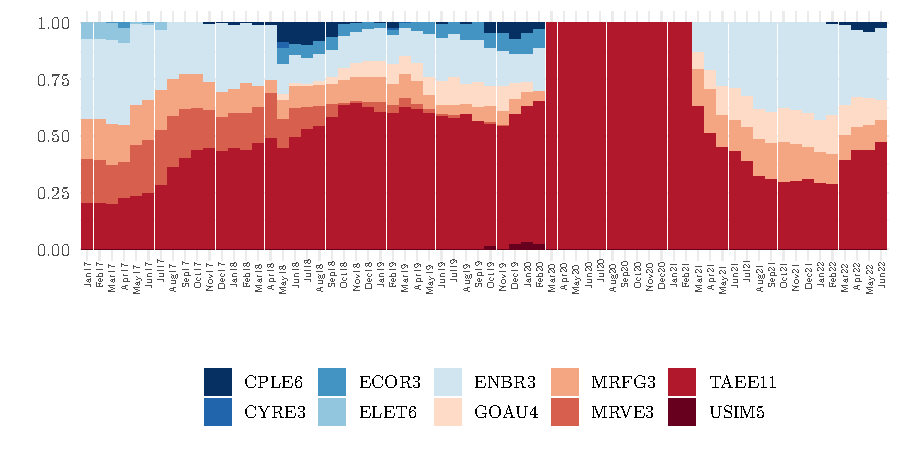
\includegraphics{figures/WeigthMVPLow10.pdf}}
% 		\subfigure[Risks]{\includegraphics{figures/RiskMVPLow10.pdf}}
% 	\end{subfigmatrix}
% 	\caption{Monthly distribution of MVP.}
% 	\label{fig:totalRiskMVP}
% 	%\end{adjustwidth}
% \end{figure}


% % A RPP has the weights distributed with the purpose of having a uniform risk distribution, Figure \ref{fig:totalRiskPPP} shows the distribution of weights and risks in our backtest study.

% \begin{figure}[H]
% 	%\begin{adjustwidth}{2.2cm}{2.2cm}
% 	\begin{subfigmatrix}{2}
% 		\subfigure[Weigths]{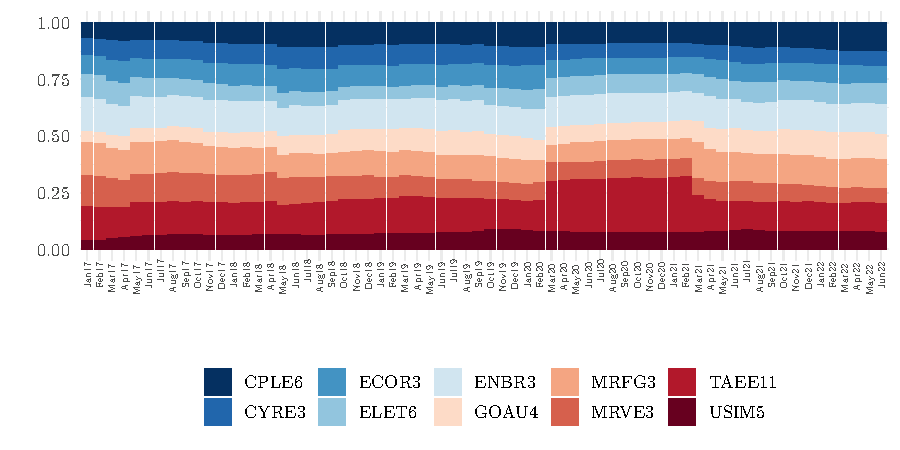
\includegraphics{figures/WeigthRPPLow10.pdf}}
% 		\subfigure[Risks]{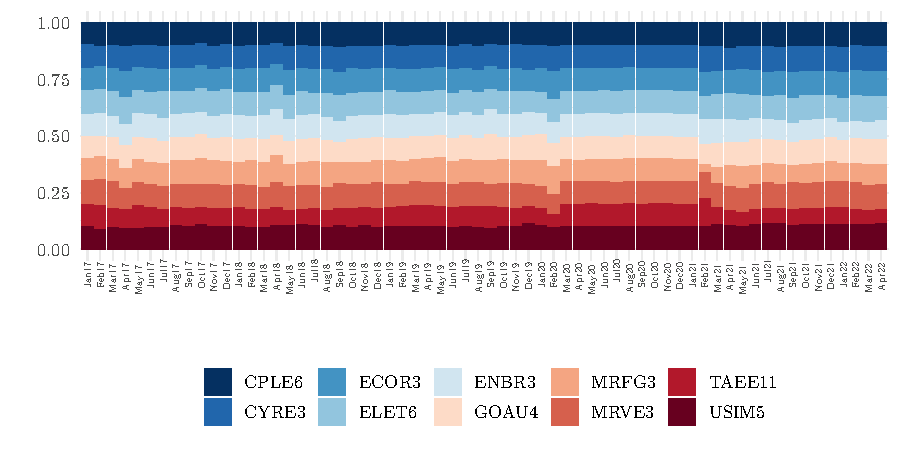
\includegraphics{figures/RiskRPPLow10.pdf}}
% 	\end{subfigmatrix}
% 	\caption{Monthly distribution of RPP.}
% 	\label{fig:totalRiskPPP}
% 	%\end{adjustwidth}
% \end{figure}

% % The total return of the RPP was greater than the MVP in the period studied. While MVP had a total return of 52\%, the accumulated RPP return was 119\% (44\% higher than the MVP).

% \begin{figure}[H]
% 	\centering
% 	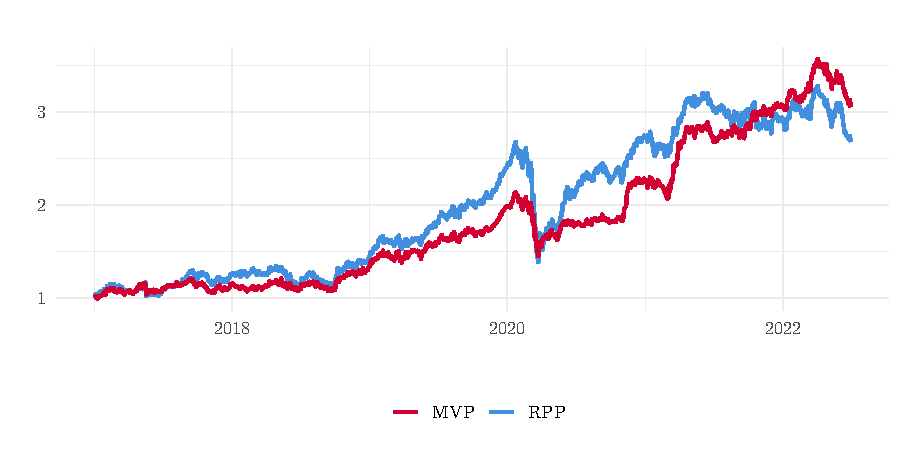
\includegraphics{figures/retornoLow10.pdf}
% 	\caption{MVP and RPP accumulated returns: January 2017 $-$ June 2022.}
% 	\label{fig:retornoRPPMVP}
% \end{figure}

% % The MVP volatility was slightly smaller than the RPP. However, considering the zero risk-free rate, the RRP Sharpe ratio was bigger than the MVP.

% \begin{table}
      \centering
      \begingroup
      \fontsize{9}{9}
      \selectfont 
\begin{tabular}{>{}lrr}
\toprule
  & MVP & RPP\\
\midrule
\textbf{Annualized Return} & 0.2287 & 0.1993\\
\textbf{Annualized Std Dev} & 0.2085 & 0.2756\\
\textbf{Annualized Sharpe (Rf=0\%)} & 1.0964 & 0.7231\\
\bottomrule
\end{tabular} \caption{Annualized Returns: Jan17 - Jun22}
      \label{tab: Low10 }  
      \endgroup{}
      \end{table}


% % We remind that after 2020, due to the COVID-19 pandemic, the volatility of all assets has exploded, so we separate two period in our study, from 2017 until 2019 and after 2020. We may observe that the RPP performed much better (135\% gain) than the MVP (79\% gain) in the period between January 2017 and December 2019. Besides, MVP had a great annualized Sharpe ratio of 1.20, however, lower than RPP annualized Sharpe ratio (1.58).

% \begin{table}
      \centering
      \begingroup
      \fontsize{9}{9}
      \selectfont 
\begin{tabular}{>{}lrr}
\toprule
  & MVP & RPP\\
\midrule
\textbf{Annualized Return} & 0.2601 & 0.3435\\
\textbf{Annualized Std Dev} & 0.1918 & 0.2273\\
\textbf{Annualized Sharpe (Rf=0\%)} & 1.3565 & 1.5114\\
\bottomrule
\end{tabular} \caption{Annualized Returns: Jan17 - Dez19}
      \label{tab: Low101 }  
      \endgroup{}
      \end{table}

% \begin{figure}[H]
% 	%\begin{adjustwidth}{2.2cm}{2.2cm}
% 	\begin{subfigmatrix}{2}
% 		\subfigure[January 2017 $-$ December 2019.]{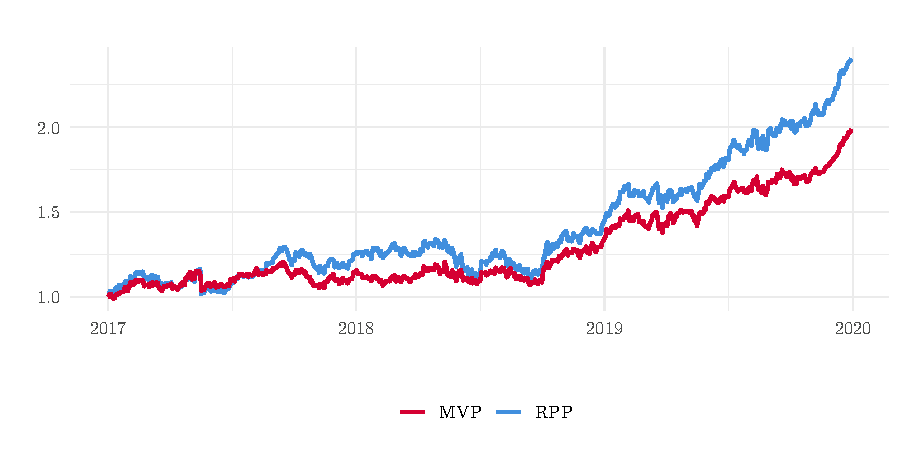
\includegraphics{figures/retornoLow101.pdf}}
% 		\subfigure[January 2020 $-$ June 2022.]{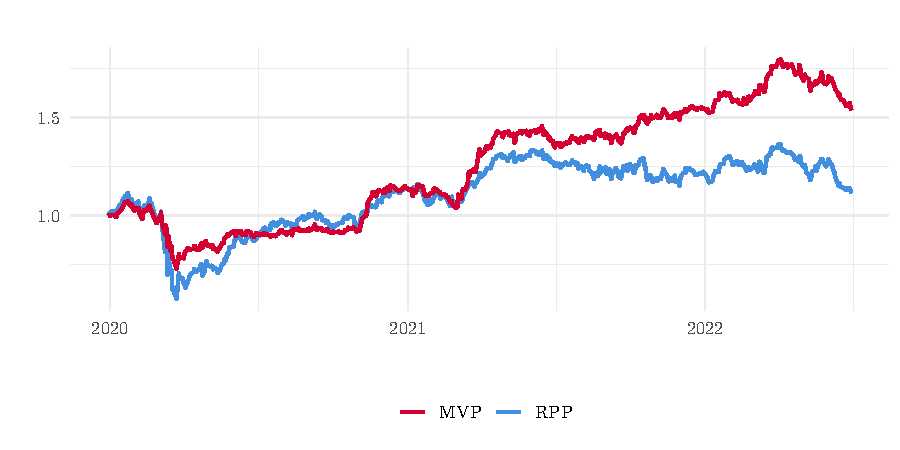
\includegraphics{figures/retornoLow102.pdf}}
% 	\end{subfigmatrix}
% 	\caption{MVP and RPP accumulated returns.}
% 	\label{fig:retornoRPPMVP12}
% 	%\end{adjustwidth}
% \end{figure}

% % From January 2020 to June 2022, MVP exhibited an accumulated $15.2\%$ loss, while RPP reduced the loss to only $6.8\%$. Despite the loss in the period, the RPP improved the protection of the invested capital.

% \begin{table}
      \centering
      \begingroup
      \fontsize{9}{9}
      \selectfont 
\begin{tabular}{>{}lrr}
\toprule
  & MVP & RPP\\
\midrule
\textbf{Annualized Return} & 0.1917 & 0.0456\\
\textbf{Annualized Std Dev} & 0.2273 & 0.3246\\
\textbf{Annualized Sharpe (Rf=0\%)} & 0.8432 & 0.1403\\
\bottomrule
\end{tabular} \caption{Annualized Returns: Jan20 - Jun22}
      \label{tab: Low102 }  
      \endgroup{}
      \end{table}

% % In our study, the RPP had a superior performance when compared to the MVP, both in high and low moments. Clearly, this study is not conclusive, but simply an example of the use of Algorithm~\ref{Alg:GeneralSeach}.

